\documentclass[twocolumn,9pt]{ltjsarticle}

\usepackage[top=15mm,bottom=15mm,left=20mm,right=20mm,columnsep=10mm]{geometry}
\usepackage[haranoaji,nfssonly]{luatexja-preset}
\usepackage{graphicx}
\usepackage{titlesec}
\usepackage{url}

\usepackage{multirow}    % セル結合用
\usepackage{tabularx}    % 表用&カラムサイズ指定

%% カラムサイズの指定用 %%
\newcolumntype{C}[1]{>{\centering\arraybackslash}p{#1}}
\newcolumntype{L}[1]{>{\raggedright\arraybackslash}p{#1}}
\newcolumntype{R}[1]{>{\raggedleft\arraybackslash}p{#1}}

\title{【実験】周期的な通信とステータスコードの関係について}
\author{山下 尚彦}
\date{\today}

\begin{document}
\maketitle

\section{はじめに}
本研究メモでは, データセットBOS\_2016に対する実験の結果で明らかになった周期的な通信とそのHTTPレスポンスステータスコード(以下ステータスコード)についてまとめる. 

\section{BOS\_2016の検体と挙動, 通信について}
本章では, BOS\_2016について報告した論文\cite{weko_175829_1}からBOS\_2016の挙動と通信について述べる. 

表\ref{tab:bos2016}はBOS\_2016の検体と挙動, C2サーバとの通信についてまとめたものである. BOS\_2016にはマルウェア検体を実行できたもの(Case e04, e12, e20, e70, e435)と実行できなかったもの(Case e43)がある. また, 実行できた検体の中でC2サーバと正常に通信できたのはe04のみで, それ以外の検体ではC2サーバなどのエラーやSYNパケットのみを送信するなど, C2サーバと正常に通信できなかった. 

\begin{table}[htbp]
    \centering
    \caption{BOS\_2016の検体の挙動と通信について}

    \begin{tabular}{C{20mm}L{15mm}L{30mm}}
        %% カラム名 %%
        \hline
        Case & 挙動 & 通信 \\
        \hline \hline
        %% データ %%
        e04 & 動作 & 攻撃活動を観測 \\ \hline
        e12\par e20 & 動作 & C2サーバとの通信が成立しない(403, 404, 503) \\ \hline
        e43 & 実行不可 & 通信発生せず \\ \hline
        e70\par e435 & 動作 & C2サーバへSYNパケットのみ送信 \\
        \hline
    \end{tabular}

    \label{tab:bos2016}
\end{table}

\section{結果}
本章では, LombScargleピリオドグラムでBOS\_2016を周波数解析した結果から周期的な通信とステータスコードについて述べる. なお, 本研究メモではマルウェア検体が動作しC2サーバとのTCPコネクションを確立したが, HTTPのステータスコードが403(Forbidden),404(Not Found), 503(Service Unavailable)などでC2サーバとの通信が成立しなかったe12とe20と, マルウェアが活動しTCP SYNパケットをC2サーバに送信したが, TCPコネクションを確立できなかったe70, e435の結果について記述する. 

\subsection{Case e12}
e12はC2サーバとTCPコネクションを確立できたが, C2サーバとの通信が成立しなかった事例で, C2サーバのIPアドレスは\ast\ast\ast.56.81.119と\ast\ast\ast.76.86.155である. 表\ref{tab:e12_ip}から2016年2月12日にC2サーバのIPアドレスを両方とも検出することができた. 図\ref{fig:e12_result1}は\ast\ast\ast.56.81.119との, 図\ref{fig:e12_result2}は\ast\ast\ast.76.86.155との通信回数とLomb-Scargleピリオドグラムによる解析結果を表した図である. 

表\ref{tab:e12_status_code}は, C2サーバからの返ってきたステータスコードの種類と数の関係を表した表である. 

\begin{table}[htbp]
    \centering
    \caption{e12で周期的な通信を示した受信先IP}

    \begin{tabular}{|c||c|l|}
        \hline
        DATE & PERIODIC & IP ADDRESS \\
        \hline \hline
        20160212 & 99.9\% & \begin{tabular}{l}
                               \ast\ast\ast.79.197.250 \\
                               \ast\ast\ast.32.241.24  \\
                               \ast\ast\ast.56.81.119  \\
                               \ast\ast\ast.76.86.155
                            \end{tabular} \\ \hline
        20160215 & 99.9\% & \begin{tabular}{l}
                               \ast\ast\ast.76.4.147   \\
                               \ast\ast\ast.59.139.27  \\
                               \ast\ast\ast.59.160.60  \\
                               \ast\ast\ast.213.168.19
                            \end{tabular} \\ \hline
    \end{tabular}

    \label{tab:e12_ip}
\end{table}

\begin{figure}[htbp]
    \centering

    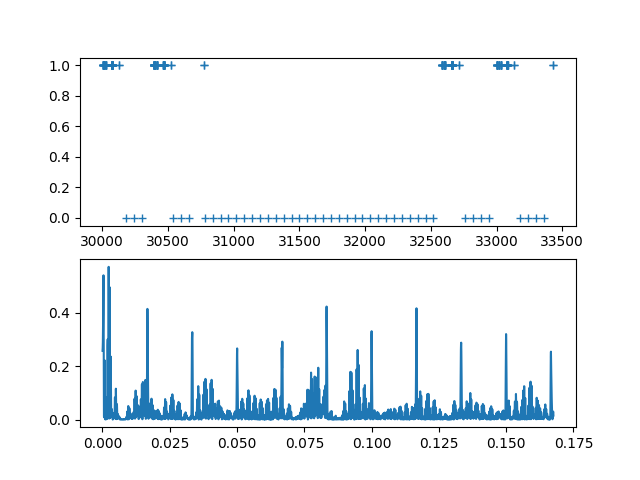
\includegraphics[width=7.5cm]{images/【実験】通信時間の粒度を高めたデータでの周期分析結果/e12/c2-1.png}

    \caption{\ast\ast\ast.56.81.119の通信回数と解析結果}
    \label{fig:e12_result1}
\end{figure}

\begin{figure}[htbp]
    \centering

    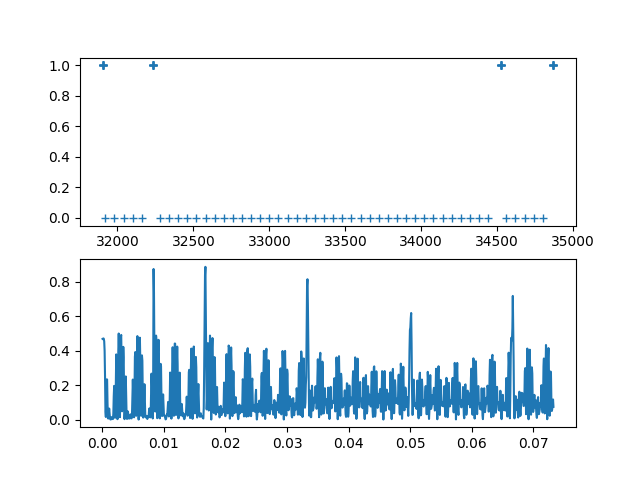
\includegraphics[width=7.5cm]{images/【実験】通信時間の粒度を高めたデータでの周期分析結果/e12/c2-2.png}

    \caption{\ast\ast\ast.76.86.155の通信回数と解析結果}
    \label{fig:e12_result2}
\end{figure}

\begin{table}[htbp]
    \centering
    \caption{ステータスコードの出現回数}

    \begin{tabular}{|l||c|c|}
        \hline
        IP ADDRESS & 200(OK) & 403(Forbidden) \\
        \hline \hline
        \ast\ast\ast.56.81.119 & 4 & 16 \\ \hline
        \ast\ast\ast.76.86.155 & 4 & 3  \\ \hline
    \end{tabular}

    \label{tab:e12_status_code}
\end{table}

\subsection{Case e20}
e20もe12と同様に, C2サーバとTCPコネクションを確立できたが通信が成立しなかった事例である. e20のC2サーバのIPアドレスは\ast\ast\ast.81.81.137である. しかし表\ref{tab:e20_ip}から分かるように, 今回の実験ではC2サーバとの周期的な通信を検出できなかった. 図\ref{fig:e20_count}はe20のマルウェア検体とC2サーバとの通信時間と回数の関係を表す図である. 

\begin{table}[htbp]
    \centering
    \caption{e20で周期的な通信を示した受信先IP}

    \begin{tabular}{|c||c|l|}
        \hline
        DATE & PERIODIC & IP ADDRESS \\
        \hline \hline
        20160215 & 99.9\% & \begin{tabular}{l}
                               \ast\ast\ast.32.1.160   \\
                               \ast\ast\ast.107.4.50   \\
                               \ast\ast\ast.58.221.163
                            \end{tabular} \\ \hline
        20160216 & 99.9\% & \begin{tabular}{l}
                               \ast\ast\ast.118.6.83
                            \end{tabular} \\ \hline
        20160218 & 99.9\% & \begin{tabular}{l}
                               \ast\ast\ast.32.1.160   \\
                               \ast\ast\ast.36.102.106 \\
                               \ast\ast\ast.113.237.189
                            \end{tabular} \\ \hline
    \end{tabular}

    \label{tab:e20_ip}
\end{table}

\begin{figure}[htbp]
    \centering

    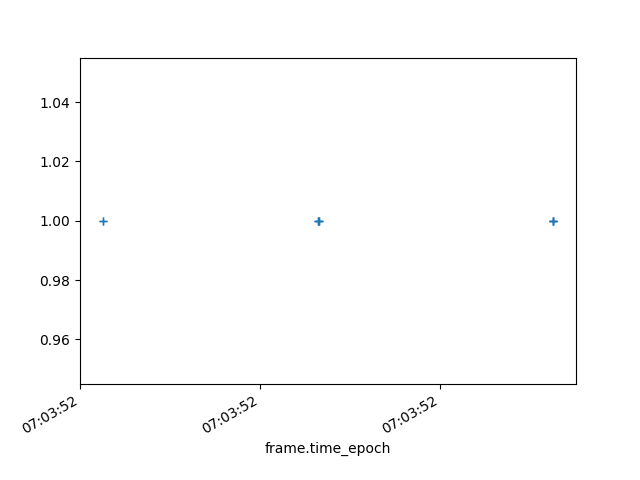
\includegraphics[width=7.5cm]{images/【実験】通信時間の粒度を高めたデータでの周期分析結果/e20/count.png}

    \caption{\ast\ast\ast.81.81.137の通信回数}
    \label{fig:e20_count}
\end{figure}

\subsection{Case e70, e435}
マルウェアが動作したがTCPコネクションを確立できなかったe70とe435のそれぞれのC2サーバのIPアドレスは, \ast\ast\ast.106.20.192と\ast\ast\ast.24.93.253である. 表\ref{tab:e70_ip}と表\ref{tab:e435_ip}から実験によってC2サーバの周期的な通信を検出できたことが分かる. 

e70とe435はC2サーバとTCPコネクションを確立できなかったため, ステータスコードを取得することができなかった. 

\begin{table}[htbp]
    \centering
    \caption{e70で周期的な通信を示した受信先IP}

    \begin{tabular}{|c||c|l|}
        \hline
        DATE & PERIODIC & IP ADDRESS \\
        \hline \hline
        20160215 & 99.9\% & \begin{tabular}{l}
                               \ast\ast\ast.32.101.160  \\
                               \ast\ast\ast.165.83.176  \\
                               \ast\ast\ast.21.181.152  \\
                               \ast\ast\ast.208.153.9   \\
                               \ast\ast\ast.106.149.145 \\
                               \ast\ast\ast.106.20.192  \\
                               \ast\ast\ast.106.253.18
                            \end{tabular} \\ \hline
        20160216 & 99.9\% & \begin{tabular}{l}
                               \ast\ast\ast.32.101.160  \\
                               \ast\ast\ast.165.83.176  \\
                               \ast\ast\ast.21.181.152  \\
                               \ast\ast\ast.208.153.9   \\
                               \ast\ast\ast.106.149.145 \\
                               \ast\ast\ast.106.20.192  \\
                               \ast\ast\ast.106.253.18
                            \end{tabular} \\ \hline
        20160217 & 99.9\% & \begin{tabular}{l}
                               \ast\ast\ast.32.101.160  \\
                               \ast\ast\ast.165.83.176  \\
                               \ast\ast\ast.21.181.152  \\
                               \ast\ast\ast.208.153.9   \\
                               \ast\ast\ast.106.149.145 \\
                               \ast\ast\ast.106.20.192  \\
                               \ast\ast\ast.106.253.18
                            \end{tabular} \\ \hline
        20160218 & 99.9\% & \begin{tabular}{l}
                               \ast\ast\ast.32.101.160  \\
                               \ast\ast\ast.165.83.176  \\
                               \ast\ast\ast.21.181.152  \\
                               \ast\ast\ast.208.153.9   \\
                               \ast\ast\ast.106.149.145 \\
                               \ast\ast\ast.106.20.192  \\
                               \ast\ast\ast.106.253.18
                            \end{tabular} \\ \hline
    \end{tabular}

    \label{tab:e70_ip}
\end{table}

\begin{table}[htbp]
    \centering
    \caption{e435で周期的な通信を示した受信先IP}

    \begin{tabular}{|c||c|l|}
        \hline
        DATE & PERIODIC & IP ADDRESS \\
        \hline \hline
        20160328 & 99.9\% & \begin{tabular}{l}
                               \ast\ast\ast.24.93.253  \\
                               \ast\ast\ast.213.168.10
                            \end{tabular} \\ \hline
        20160329 & 99.9\% & \begin{tabular}{l}
                               \ast\ast\ast.24.93.253
                            \end{tabular} \\ \hline
        20160330 & 99.9\% & \begin{tabular}{l}
                               \ast\ast\ast.24.93.253
                            \end{tabular} \\ \hline
    \end{tabular}

    \label{tab:e435_ip}
\end{table}

\begin{figure}[htbp]
    \centering

    \includegraphics[width=7.5cm]{images/【実験】通信時間の粒度を高めたデータでの周期分析結果/e70/c2.png}

    \caption{\ast\ast\ast.106.20.192の通信回数と解析結果}
    \label{fig:e70_result}
\end{figure}

\begin{figure}[htbp]
    \centering

    \includegraphics[width=7.5cm]{images/【実験】通信時間の粒度を高めたデータでの周期分析結果/e435/c2.png}

    \caption{\ast\ast\ast.24.93.253の通信回数と解析結果}
    \label{fig:e435_result}
\end{figure}

\section{考察}
本章では, 実験の結果から考察を行う. 

今回の実験はC2サーバとTCPコネクションを確立できたが通信が成立しなかったe12, e20とC2サーバとのTCPコネクションが確立できず, TCP SYNパケットを送信し続けたe70, e435の通信観測データをLomb-Scargleピリオドグラムによって解析した. 実験の結果, e12とe70, e435でC2サーバとの周期的な通信を検出できたが, e20では検出した周期的な通信の中にC2サーバとの通信が含まれていなかった. これは図\ref{fig:e20_count}から分かるように, 短時間に3回しか通信を行っていないことが原因と考えられる. 

また, C2サーバとTCPコネクションを確立でき, かつ, C2サーバとの周期的な通信を検出できたe12のステータスコードに関して調査を行った結果, \ast\ast\ast.56.81.119からのレスポンスは大半が403(Forbidden)で, たまにリクエストが正常に完了したことを示す200(OK)が返ってきた. そのため, e12とC2サーバ\ast\ast\ast.56.81.119は正常に通信ができていない可能性が高いため, 対処優先度は低くできると考えられる. 一方で\ast\ast\ast.76.86.155の場合, 403(Forbidden)よりも200(OK)を示すレスポンスが多かったため, 対処優先度は高くする必要がある. e70, e435はステータスコードを取得できなかったためC2サーバとTCPコネクションを確立できなかった可能性が高いため, 対処優先度を低くできると思われる. 

\section{おわりに}
本研究メモでは, データセットBOS\_2016をLomb-Scargleピリオドグラムによって解析し, C2サーバとの通信を含めた周期的な通信を検出し, C2サーバからのHTTPレスポンスステータスコードについて調査を行った. 

Lomb-Scargleピリオドグラムによる解析の結果, e12, e70, e435でC2サーバとの周期的な通信を検出することができたが, e20のように短時間に数回しかC2サーバと通信を行った事例ではLomb-Scargleピリオドグラムによる検出は困難であることが分かった. 

ステータスコードによる対処優先度の決定に関して, TCPコネクションを確立できた事例ではステータスコードを取得することができたため対処優先度を決定することができた. また, TCPコネクションを確立できなかった事例であっても, C2サーバとの周的な通信を検出することができたため, 優先度を低いものに決定できた. 

\bibliographystyle{junsrt}
\bibliography{DB}
\end{document}